\documentclass[11pt,parskip]{scrartcl}
\usepackage[ngerman]{babel}

% For XeTeX %%%%%%%%%%%%%%%%%%%%%%%%%%%%%%%%%%%%%%%%%%%%%%%%%%%%%%%%%%%%%%%%%%%%
\usepackage{fontspec}
\setromanfont{Linux Libertine O}
\setsansfont{Linux Biolinum O}

% For pdfTeX %%%%%%%%%%%%%%%%%%%%%%%%%%%%%%%%%%%%%%%%%%%%%%%%%%%%%%%%%%%%%%%%%%%
%\usepackage[T1]{fontenc}
%\usepackage{inputenc}
%\usepackage{mathpazo}

% Packages %%%%%%%%%%%%%%%%%%%%%%%%%%%%%%%%%%%%%%%%%%%%%%%%%%%%%%%%%%%%%%%%%%%%%
%\usepackage{biblatex}
\usepackage{amsmath}
\usepackage[a4paper]{geometry}
\usepackage{graphicx}
\usepackage{xcolor}
\usepackage{microtype}
\usepackage{booktabs}
\usepackage[colorlinks=false, pdfborder={0 0 0 }]{hyperref}
\usepackage{cleveref}
\usepackage[autostyle=true,german=quotes]{csquotes}
\usepackage{blindtext}
\usepackage{listings}

% Options %%%%%%%%%%%%%%%%%%%%%%%%%%%%%%%%%%%%%%%%%%%%%%%%%%%%%%%%%%%%%%%%%%%%%%
\widowpenalty=10000
\clubpenalty=10000


% Begin of document %%%%%%%%%%%%%%%%%%%%%%%%%%%%%%%%%%%%%%%%%%%%%%%%%%%%%%%%%%%%
\begin{document}


% Titlepage %%%%%%%%%%%%%%%%%%%%%%%%%%%%%%%%%%%%%%%%%%%%%%%%%%%%%%%%%%%%%%%%%%%%
%
\begin{titlepage}
  \begin{sffamily}
    {\scshape\LARGE \textcolor{gray}{Universität Hamburg}\par}
    {\scshape\Large \textcolor{gray}{Projektarbeit Interactive Visual
        Computing}\par}
    \vspace{2.5cm}
    \centering
    {\huge\bfseries Babytux\par}
    {\large\bfseries Ein Povray-Film über das Erwachsenwerden eines Pinguins\par}
    \vspace{1.5cm}
    {\Large\itshape \textcolor{darkgray}{
        Lemme, Inga \quad{}
        Ort, Thomas \quad{}
        Remmels, Melanie
      }\par
    }
    \vfill
    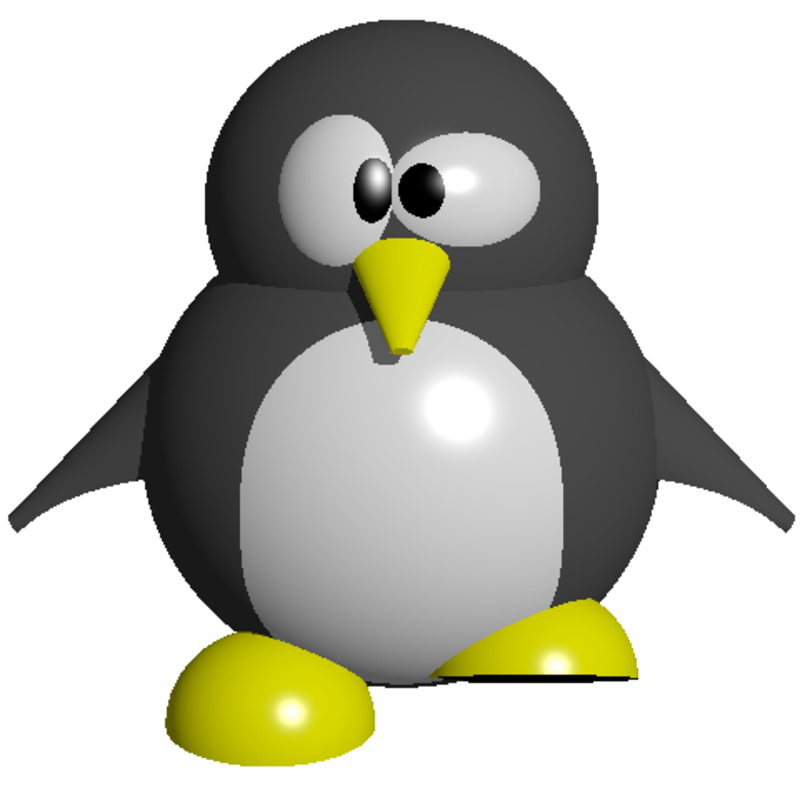
\includegraphics[width=0.20\textwidth]{./fig/ourtux.pdf}\par\vspace{1cm}
    \vfill
    % Bottom of the page
    {\large \today\par}
  \end{sffamily}
\end{titlepage}
%
% End of Titlepage %%%%%%%%%%%%%%%%%%%%%%%%%%%%%%%%%%%%%%%%%%%%%%%%%%%%%%%%%%%%%


\newpage
\tableofcontents
\newpage


\section{Projektidee}
Vorlage für die Hauptfigur des hier beschriebenen Films ist das Maskottchen des
freien Kernels \emph{Linux}. Dieses stellt einen Pinguin dar und wird kurz
\emph{Tux} genannt. \emph{Tux} wurde im Jahr 1996 von \emph{Larry Ewing} mit
der Bildbearbeitungssoftware \emph{GIMP} entworfen und steht seitdem zur freien
Verfügung für die Gemeinde. Er darf nach Belieben verwendet und verändert
werden, solange auf Nachfrage sowohl Urheber\footnote{lewing@isc.tamu.edu} als
auch das verwendete Programm genannt werden. \cite{ewing}

Die Idee, dass das Logo ausgerechnet einem Pinguin nachempfunden ist, stammt
von \emph{Linus Torvalds}, dem Gründer von Linux. Laut \emph{Jeff Ayers}, einem
Linuxentwickler, besitzt \emph{Torvalds} eine Affinität für
\enquote{\emph{flugunfähige, fette Wasservögel}}, sodass letztlich der Entwurf
von \emph{Ewing} übernommen wurde. Eine weitere Anekdote, die zur Auswahl des
Pinguins beigetragen hat stammt von einem Erlebnis \emph{Torvalds} in einem
Aquarium in Canberra, Australien. Dort wurde er von einem Pinguin gebissen und
sei seitdem mit der Krankheit \emph{Penguinitis} infiziert:

\begin{quote}
  \enquote{Penguinitis makes you stay awake at nights just thinking about
    penguins and feeling great love towards them.} \cite{tuxstory}
\end{quote}

Es gibt inzwischen unzählige Versionen des Maskottchens, in dieser
Arbeitsgruppe haben wir uns an einer modernen und jungen Version des Pinguins
orientiert wie in Abbildung \ref{fig:overlord59tux} zu sehen.

\begin{figure}[htbp]
  \centering
  
\includegraphics[width=0.3\textwidth]{./fig/overlord59tux.pdf}
  \caption{
    Die Hauptfigur des Filmes wurde nach diesem Vorbild entwickelt. Das
    gezeigte Modell stammt vom Autor \emph{Overlord59} und wurde unter
    \emph{Creative Commons BY-NC-SA} veröffentlicht.
    \emph{
      (Quelle: \url{http://tux.crystalxp.net/de.id.1568-overlord59-overlord59-tux-g2.html)}
    }
  }
  \label{fig:overlord59tux}
\end{figure}


\subsection{Plot des Films}
Zu Beginn des Films ist zunächst ein Ei zu sehen, welches immer größere Risse
bekommt und anschließend ein Stück aus dem Ei heraus bricht. Aus dem
heraus gebrochenen Stück schauen die Augen des Tux.

Der obere Teil des Eis bricht auf und letztlich schlüpft der Tux. Anschließend
entdeckt der Pinguin, dass er Füße, Flügel und seinen Schwanz bewegen kann.
Nachdem er sich etwas umsieht beginnt er seine Gegend zu erkunden und läuft
los.

Im weiteren Verlauf wird ein Zeitraffer-Effekt eingesetzt. Der Tux wächst
langsam und entdeckt dabei die schönen und schwierigen Dinge des Lebens.


\newpage

\section{Statischer Aufbau der Figuren}
Im Folgenden wird beschrieben mittels welcher povray-Funktionen und Objekte die
einzelnen Figuren, Requisiten und Szenenbilder des Films erstellt wurden.


\subsection{Konstruktion der Umgebung}
In der Datei \texttt{environment.pov} wurde die Umgebung konstruiert, sodass
diese in die jeweiligen Sequenzen inkludiert werden können.


\subsection{Aufbau des Pinguineis}
Die Grundstruktur des Eis wurde von der Vorgängergruppe (Teil 1) übernommen
und an unseren Film angepasst. Dazu wurden jeweils für den oberen Teil und den
unteren Teil des Eis ein weiteres etwas kleineres Ei-Objekt erzeugt und mittels
\texttt{difference} vom größeren Objekt abgezogen. Dadurch wird das Ei von
innen hohl. Damit das jeweilige Objekt auch als hohl erkannt wird, wurde das
innere Objekt minimal nach oben bzw. nach unten verschoben.

\begin{lstlisting}
  difference{
    object{ Egg_lowerpart }
    object{
      Egg_lowerpart
      translate <0, 0.1, 0>
      scale <0.9, 0.9, 0.9>
    }
  }
\end{lstlisting}


\subsection{Aufbau der Hauptfigur}


\subsubsection{Körper}
Zu allererst werden die Proportionen als \texttt{declare}-Anweisung festgelegt.
Um die Proportionen unabhängig von der Größe des Tux gleich zu halten, wird
nur die Höhe \texttt{tuxheight} variabel gehalten. Die anderen Größen wie
\texttt{tuxwidth} oder \texttt{radiustummy} werden mit \texttt{tuxheight}
verrechnet.

Der Grundaufbau des Tux besteht aus zwei Grundkugeln, in povray \texttt{sphere}
genannt. Einer unteren großen Kugel für den Unterleib und einer etwas kleineren
Kugel für den Kopf oberhalb. Der Unterleib besteht zunächst aus \emph{einer}
Kugel. Zur Realisierung des weißen Bauches existieren zwei weitere
\texttt{sphere}-Objekte, deren Schnittmenge (\emph{intersection}) anschließend
mit der großen Kugel vereinigt wird (\emph{union}).
%
\begin{lstlisting}
  union{
    intersection{
      sphere{ 0, radiustummy }
      sphere{ 0, radiustummy }
      scale <0.6, 1.5, 0.25>
      translate <0, 0, -radiustummy + 0.1>
    }
    pigment{ White }
    sphere{
      0, radiustummy
      pigment{ Gray10 }
    }
  }
\end{lstlisting}
%
Die weiße Schnittmenge ist mit den Funktionen \texttt{scale} und
\texttt{translate} so verschoben und skaliert, dass der vordere Teil der
Hauptkugel in den richtigen Proportionen weiß erscheint. Sowohl Kopf, als auch
Unterleib sind in einer \texttt{declare}-Anweisung als \texttt{head} und
\texttt{tummy} global geltend gemacht. So können diese direkt angesprochen
werden, ohne den Code immer wieder neu reproduzieren zu müssen.

Der Kopf des Pinguins ist mit einer \texttt{sphere} generiert, die zwei Drittel
der Größe des Unterleibs beträgt. In den Kopf sind Augen mit schwarzen Pupillen
eingelassen. Zunächst ist die Pupille in einer \texttt{declare}-Anweisung
festgelegt. Sie besteht wie der Bauch aus der Schnittmenge zweier Kugeln. Die
beiden Augen sind in \texttt{LeftEye} und \texttt{RightEye} deklariert. Hier
sind die Pupillen als Objekt mit einem weiteren \texttt{sphere}-Objekt
vereinigt (\texttt{union}).

Der Schnabel des Tux ist mittels eines \texttt{cone}-Objektes realisiert.
Hierbei sind Zentrum und Radius der beiden Enden, sowie die Skalierung des
gesamten Objektes so gewählt, dass ein flach gedrückter Kegel entsteht.

\subsubsection{Gliedmaßen}
Der Tux besteht weiterhin aus zwei Füßen und zwei Flügeln.


\subsection{Utensilien}
Der Tux ist in diesem Film ein weibliches Jungtier, daher wurde eine Schleife
und ein Schnuller konstruiert.


\subsubsection{Bewegliche Gliedmaßen}


\newpage

\section{Aufbau der einzelnen Animationssequenzen}


\subsection{Titelsequenz}


\subsection{Sequenz 1: Schlüpfen des Tux}
Zunächst bekommt das Ei einen Riss. Als nächstes bricht ein Stück aus dem Ei
heraus und die Augen des Tux erscheinen aus dem dunklen Inneren des Eis. Zur
Realisierung dieser Szene wurde ein Objekt \texttt{Crack} erstellt.
\texttt{Crack} besteht aus mehreren quadratischen \texttt{box}-Objekten die
ineinander verdreht sind.
%
\begin{lstlisting}
  union{
    box{
      <-0.5, 0, -0.5>
      <0.5, 0.1, 0.5>
    }
    box{
      <-0.5, 0, -0.5>
      <0.5, 0.1, 0.5>
      rotate <5, 20, 10>
    }
    ...
  }
\end{lstlisting}
%
Dieses Objekt wurde so klein erstellt, dass es in das Ei-Objekt passt.
Anschließend wurde das \texttt{crack}-Objekt abhängig von der Zeit in der x- und
z-Richtung größer skaliert und eine Differenz zum Ei-Objekt gebildet. Die
Animation zeigt im Ergebnis einen Riß, der sich immer mehr vergrößert und am
Ende zwei Ei-Hälften erscheinen.
%
\begin{lstlisting}
  ...
\end{lstlisting}
%

\subsection{Sequenz 2: Babytux entdeckt seine beweglichen Gliedmaßen}


\subsection{Sequenz 3: Babytux macht erste Gehversuche}


\subsection{Abschlusssequenz}
In der Abschlusssequenz erscheint der Originaltux von Larry Ewing als
Grafik\ldots


\newpage

\section{Fertigstellung des gesamten Films}


\subsection{Zusammenfügen der einzelnen Sequenzen}


\subsection{Vertonung}


\subsection{Korrekturen}


\newpage
\addcontentsline{toc}{section}{Literatur}
\bibliographystyle{unsrt}
\bibliography{bibtux}

\end{document}
